\documentclass[]{article}

\usepackage{graphicx}
\usepackage{hyperref}

%opening
\title{SDC Pr1: Finding Lane Lines on the Road}
\author{J. Irving Vasquez-Gomez}

\begin{document}

\maketitle

%\begin{abstract}

%\end{abstract}

\section{Introduction}

In this project we are attempting to locate the lane lines of the road.

\section{Pipeline}

My approach is described in the following steps:

\begin{enumerate}
	\item Do a Gaussian filtering to remove noise.
	\item Do Canny edge detection.
	\item Eliminate irrelevant parts of the edges image with masking. 
	\item Detect large and continuous lines that have a minimum slope. See blue lines in figure \ref{fig:figure_1}. Hough transform was used to detect them. In this step only continuous lines are found, so the parameter maxLineGap is almost zero. In addition, only lines with a slope higher to 0.5 or lower to -0.5 where kept; it removes some false lines that are horizontal. 
	\item Detect large and non continuous lines that have a minimum slope. See cyan lines in figure \ref{fig:figure_1}.  I added this step because dotted lines are not detected by the previous step.
	\item Project the lines to the lower point in the image. In this step I use the slope to know the point where the line intersect the bottom border of the image.
	\item Store all the slopes and intersection points.
	\item Calculate the mean lines. In this step the lines are separated depending on their slope (negative or positive; left or right), then the slopes and projection points are averaged.
    \item Draw mean lines on the image. See figure \ref{fig:mean}.
\end{enumerate}


\begin{figure}
\centering
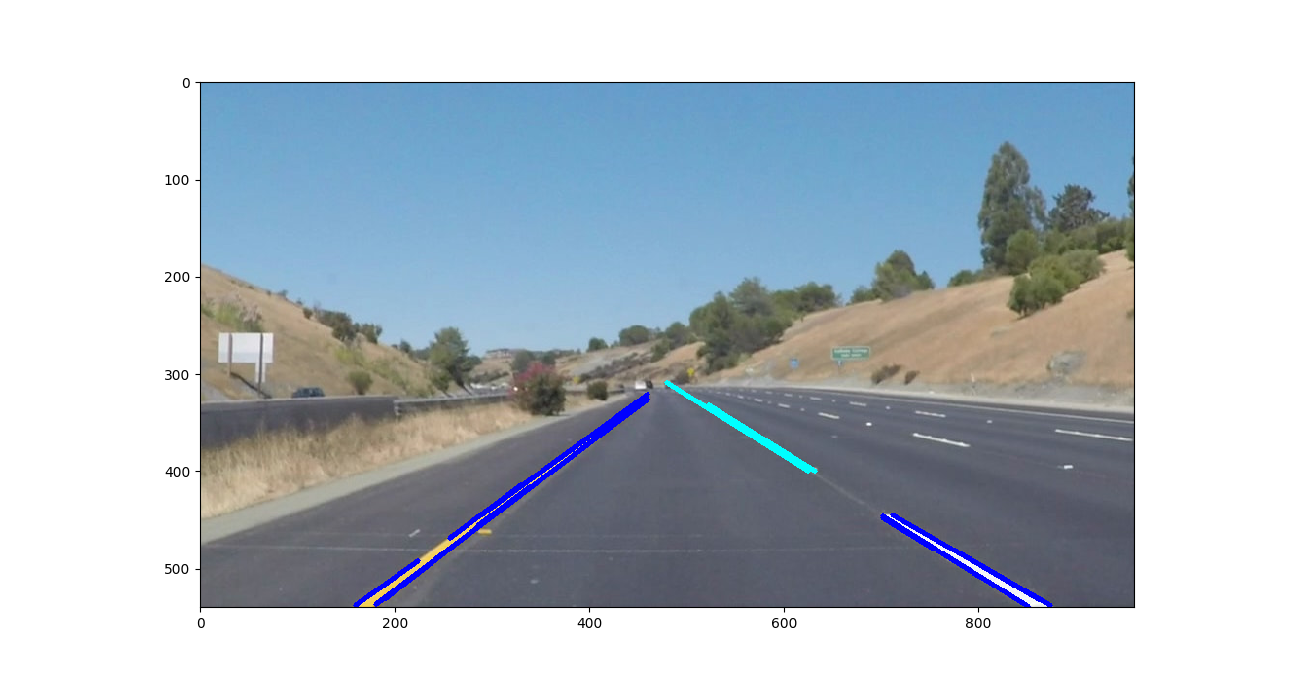
\includegraphics[width=\linewidth]{figure_1}
\caption{Detecting lane lines on example image.}
\label{fig:figure_1}
\end{figure}

\begin{figure}
\centering
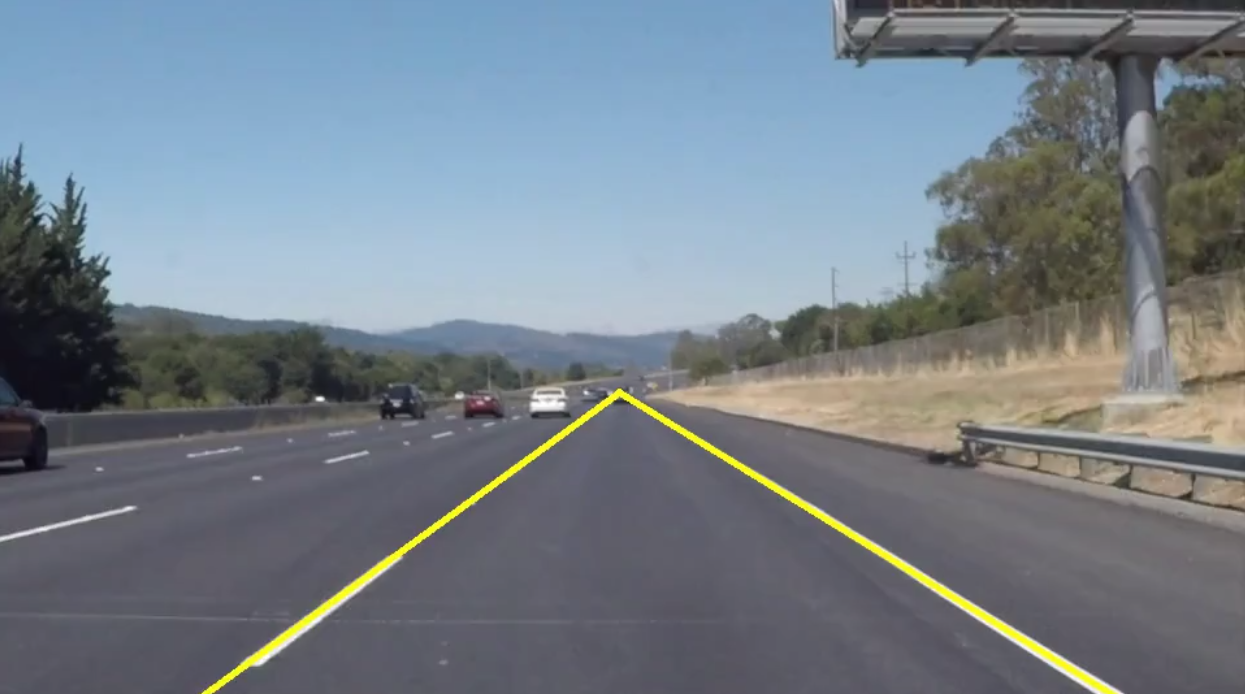
\includegraphics[width=0.7\linewidth]{mean}
\caption{Mean lines. These lines are the average of all detected lines.}
\label{fig:mean}
\end{figure}

\section{Experiments}

I tested the program on the provided videos. The results are:

\begin{itemize}
	\item \url{https://youtu.be/e-luC5kSM7g}
    \item \url{https://youtu.be/L4NEAHLeDbA}
    \item \url{https://youtu.be/xXmpXujzoTQ}
    \item \url{https://youtu.be/0inu3jldG3A}
\end{itemize}

I found that the program runs fine on the videos. However, this approach is not suitable for illumination changes or curved lines. When the illumination changes, the Canny detector needs to be adjusted. When curved lines appear in the video, my approach could not detect them or they could be estimated with a "infinite slope". 

See my test on the challenge video: \url{https://youtu.be/xtmZVbYlpFg}


\section{Improvements}

I think that illumination changes could be addressed by performing a histogram equalization. Curved lines could be detected by using a curved shape instead of lines in a generalized Hough Transformation. In addition, more information about the road can be used, for example left and right lines should converge to a point in the horizon or the lines that are closer to vertical center line of the image are more probable to be the lane lines.

\end{document}
